\documentclass{article}
\usepackage[utf8]{inputenc}
\usepackage{graphicx}
\usepackage{color}

\newenvironment{text-blue}{\color{blue}}{}
\newenvironment{text-red}{\color{red}}{}

\begin{document}

\title{Monitorização da temperatura do ar de um processo térmico \\ Trabalho prático nº3, Computação Adaptativa}
\author{Adriano Vinhas (2009106560, avinhas@student.dei.uc.pt)\\
		José Ribeiro (2008112181, jbaia@student.dei.uc.pt}
\maketitle
\clearpage

% Introdução
\section{Introdução}

\indent \indent Este trabalho, no âmbito da disciplina de Computação Adaptativa, tem como objectivo construir um sistema difuso capaz de regular a temperatura do ar através de um conjunto de entradas facultadas à rede, sendo estas alvo de transformação para corresponderem à lógica difusa. Estes valores vão ser a base da decisão de uma acção a tomar pelo sistema, que é feita através da saída.

Este objectivo foi atingido fazendo um estudo paramétrico tendo em conta os seguintes parâmetros de estudo:
\begin{itemize}
\item xxx
\item yyy
\item zzz
\item xx xx xx
\item yy yy yy
\item zz zz zz
\end{itemize}

A parte que foi mais focada na realização deste trabalho foi o estudo paramétrico feito com base nos parâmetros acima indicados. Com base nos resultados obtidos, procurámos uma solução que nos permitisse chegar à combinação dos parâmetros que minimizasse o erro da rede, para as referências que nos foram fornecidas.

\clearpage
\section{Concepção da rede difusa}
\indent \indent Nesta secção estão descritas a arquitectura da rede usada para o trabalho e a forma como o conjunto de regras da rede difusa foi definido.

A arquitectura do sistema difuso usada para o trabalho prático consiste em duas entradas, uma delas que representa o erro num instante $k$ ($e_{k}$) como a diferença entre a temperatura desejada e a temperatura do ar à saída do aquecedor nesse mesmo instante ($e_{k} = R_{k} - Y_{k}$), e a outra representando a variação do erro ($\Delta e$) como a diferença entre o erro no instante $k$ e $k-1$ ($\Delta e=e_{k}-e_{k-1}$). Em relação às saídas do sistema difuso, apenas foi definida uma, que representa a variação de potência a aplicar à grelha de aquecimento ($\Delta U$).

As restantes características da rede que são consideradas relevantes não são mencionadas aqui por terem sido alvo de estudo paramétrico.

A figura~\ref{nn_architecture} representa a arquitectura do sistema difuso usado.

\begin{figure}[!h]
  \centering
  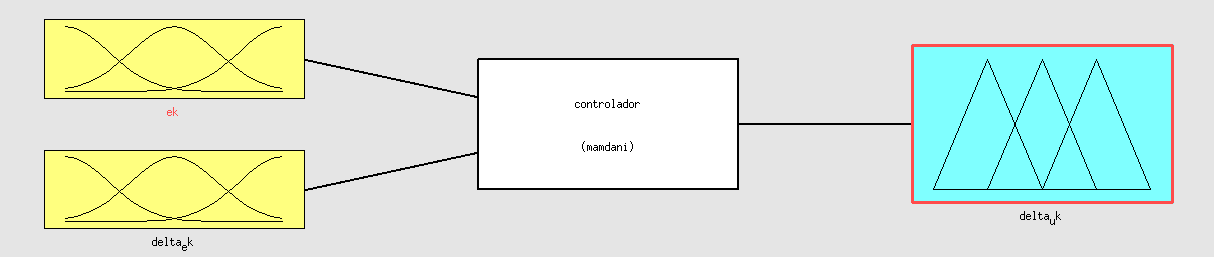
\includegraphics[width=5in]{figures/nn_architecture}
  \caption{Arquitectura da rede usada}
  \label{nn_architecture}
\end{figure}

O conjunto de regras que gerem as acções a tomar em função das entradas foi feito com especial cuidado uma vez que, entre outros factores, a definição das regras tem impacto na performance do sistema difuso.

O grupo decidiu implementar dois controladores, e definiu cada um da seguinte forma:
\begin{itemize}
\item \textbf{Controlador de 3 termos} \\
Para este controlador existem as três variáveis linguísticas mencionadas acima ($e_{k}$,$\Delta e$,$\Delta U$) e cada uma destas variavéis tem três termos linguísticos (${N,Z,P}$).

A tabela de regras para este controlador está representada na tabela~\ref{3_terms_fuzzy}.

\begin{table}[!h]
\centering
	\caption{Tabela de regras do controlador difuso de 3 termos}
	\label{3_terms_fuzzy}
	\begin{tabular}{|c|c|c|c|}
	\hline 
	$e_{k}$ $\backslash$ $\Delta e$ & \textbf{N} & \textbf{Z} & \textbf{P} \\ 
	\hline 
	\textbf{N} & N  & N & N \\ 
	\hline 
	\textbf{Z} & Z & Z & Z \\ 
	\hline 
	\textbf{P} & P & P & P \\ 
	\hline 
	\end{tabular} 
	%\vspace{-1cm}
\end{table}


\item \textbf{Controlador de 5 termos} \\
Para este controlador existem as mesmas variáveis linguísticas e cada uma destas variavéis tem cinco termos linguísticos (${NG,NP,ZO,PP,PG}$).

A tabela de regras para este controlador está representada na tabela~\ref{5_terms_fuzzy}.

\begin{table}[!h]
\centering
	\caption{Tabela de regras do controlador difuso de 5 termos}
	\label{5_terms_fuzzy}
	\begin{tabular}{|c|c|c|c|c|c|}
	\hline 
	$e_{k}$ $\backslash$ $\Delta e$ & \textbf{NG} & \textbf{NP} & \textbf{Z} & \textbf{PP} & \textbf{PG} \\ 
	\hline 
	\textbf{NG} & N  & N & N & N & N\\ 
	\hline 
	\textbf{NP} & Z & Z & Z & N & N\\ 
	\hline 
	\textbf{ZO} & P & P & P & N & N\\ 
	\hline
	\textbf{PP} & Z & Z & Z & N & N\\ 
	\hline 
	\textbf{PG} & P & P & P & N & N\\ 
	\hline 
	\end{tabular} 
	%\vspace{-1cm}
\end{table}
\end{itemize}

\clearpage
% Gráficos com os resultados. Análise e interpretação.
\section{Estudo paramétrico}
\indent \indent Nesta secção é explicada a metodologia de testes seguida para levar a cabo são apresentados os resultados do estudo paramétrico efectuado para obtenção do resultado óptimo encontrado.

Neste estudo, a ordem dos parâmetros testados torna-se fulcral para melhor explorar o espaço de combinações sem o fazer de forma exaustiva. No fim de cada variação paramétrica, o valor que optimizava as métricas usadas para medir a performance da rede neuronal era fixado na variação paramétrica seguinte. Por exemplo, após a determinação do número óptimo de neurónios para a camada escondida, esse valor era fixado para os restantes testes.

No caso do estudo do coeficiente de aprendizagem, tal não se aplica uma vez que este foi o 



\clearpage
\section{Conclusão}
\indent \indent Depois do estudo paramétrico efectuado o sistema difuso que obteve melhores resultados tinha um valor de erro/critério de \textbf{xxx}, para a entrada que nos foi fornecida para efeitos de avaliação.

Atingimos estes valores usando a seguinte parametrização:
\begin{itemize}
\item Número de termos linguísticos:
\item Tipo de funções de pertença:
\item Factores de Normalização:
\item xxx
\item yyy
\item zzz
%\item Goal (Erro de treino) ???
\end{itemize}

O gráfico que representa os valores da referência, temperatura e controlo, para o melhor sistema difuso obtido, está exibido na figura ~\ref{best_fuzzy_results}. Os valores de entrada que nos foram fornecidos tiveram em conta um intervalo de tempo de 10 segundos e um intervalo de amostragem de 0.1s.
%\begin{figure}[h!]
%  \centering
%  \includegraphics[width=5in]{figures/best_nn}
%  \caption{Performance, Sensibilidade e Especificidade da melhor rede encontrada}
%  \label{best_nn}
%\end{figure}


\end{document}
